Metals and semiconductors are composed of periodic structures of ions in 3D space -- a lattice. The outer shell electrons (usually one electron, but sometimes two or three) are so loosely bound to the original atom that are considered to be shared amongst all ions in the metal -- creating a sea of electrons. \\

\begin{figure}[H]
    \centering
    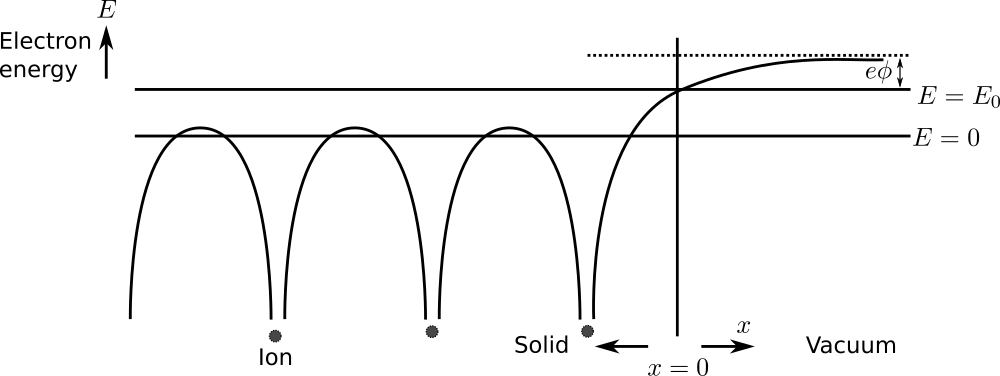
\includegraphics[width=0.8\textwidth]{figures/Theory1.png}
    \caption{Potential energy diagram for a metal. Electrons with energy $>E_0 + e\phi$ are able to escape from the surface.}
    \label{PotentialEnergy_Figure}
\end{figure}

At the boundary between the solid and vacuum (or other material) is an energy barrier. Electrons with sufficient energy to overcome this barrier can be emitted from the surface. The energy barrier is is dependent on the solid, usually around a few electron-volts. This energy barrier is the 
\textbf{work function}, $w$, of the metal -- or the amount of energy needed to remove one electron. This work function is described as,

\begin{align}
    w_0 &= e\phi
\end{align}

where $e$ is the elementary charge and $\phi$ is the electrostatic potential in the vacuum nearby the surface.\\

The free electrons of a solid have with a distribution of velocities (and thus, momenta) due to random thermal motion. The average energy is given by,

\begin{align}
    \bar{E} = \frac{1}{2} m \bar{v}^2 &= \frac{3}{2} k T \label{Kin_Tem_EnergyRelation}
\end{align}
where $m$ is the mass of the electron, $\bar{v}$ is the average velocity, $k$ is the Boltzmann constant and $T$ is the temperature of the solid.\\

However, in reality the electrons not only need sufficient energy, but must also be moving in the correct direction to leave the surface. Thus, we describe the requirement for emission in terms of momentum rather than energy. To be ejected, the electron must have enough momentum in the same direction to the surface normal. An electron moving in the $y$-direction will not be emitted from a surface at $x=0$ with surface normal in the $x$-direction (see Figure \ref{PotentialEnergy_Figure}). The electron in this example must be moving with enough momentum in the positive $x$ direction to be emitted.\\

So, as in Figure \ref{PotentialEnergy_Figure}, the electron needs energy $E = E_0 + e\phi$ to be emitted (this is the minimum requirement, and after emission the electron would have no remaining energy), and the momentum in the direction of the surface normal is,
\begin{align}
    & E_0 + e\phi = \frac{p_{x_c}^2}{2m} \\
    \intertext{Thus, the momentum in the positive $x$-direction required is,}
    & p_{x_c} = \sqrt{2m(E_0 + e\phi)} \label{CriticalMomentum}
\end{align}

The number of electrons within an infinitesimal slice of the 3D momentum is,
\begin{align}
    \frac{2}{h^3} dp_x dp_y dp_z
\end{align}

Now, using the approximation of Fermi's equation we can calculate the temperature-dependent number occupied states,
\begin{align}
    f(E) &= e^{-(E-E_0)/kT} \\
    f(\vec{p})&= e^{-(\vec{p}^2/2m - E_0)/kT}
\end{align}

So, our number of occupied states is,
\begin{align}
    N_e &= \frac{2}{h^3} e^{-(\vec{p}^2/2m - E_0)/kT}  dp_x dp_y dp_z
\end{align}

These electrons leaving the solid form an electron flux and volume current density, which we can write as,
\begin{align}
    J = e v_x N_e = \frac{e}{m} p_x N_e
\end{align}
where $v_x = p_x/m$ is the velocity in the $x$-direction and $N_e$ is the number of electrons with sufficient momenta to be emitted per unit volume that we computed above.\\

Combining the expressions previously derived, we have for current,
\begin{align}
    dJ &= \frac{2e}{mh^3} p_x e^{-((p_x^2+p_y^2 + p_z^2)/2m - E_0)/kT} dp_x dp_y dp_z \\
    J &= \frac{2e}{mh^3} \int_{p_{x_c}}^\infty dp_x \int_{-\infty}^\infty dp_y \int_{-\infty}^\infty dp_z \left[ p_x e^{-((p_x^2+p_y^2 + p_z^2)/2m - E_0)/kT} \right]
\end{align}
Solving the Gaussian integrals for $dp_y,\ dp_z$ and the exponential form integral for $dp_x$ with the value for $p_{x_c}$ derived in Equation \ref{CriticalMomentum},
\begin{align}
    J &= \frac{4\pi e m k^2 }{h^3} T^2 e^{-e\phi/kT}
\end{align}
This equation is known as the Richard-Dushman. We can simplify the constant scalar to a single, universal constant value of,
\begin{align}
    A_0 &= \frac{4\pi e m k^2 }{h^3} \\
    \intertext{which in SI units is,}
    &= 1.20173 \times 10^6 \ \text{A m$^{-2}$ K$^{-2}$}
\end{align}
So, we can write the equation in the simple form of,
\begin{align}
    J &= A_0 T^2e^{-w_0/kT} \label{Richard-Dushman_reduced}
\end{align}

However, what has been discussed so far accounts only for a solid with no applied electric field. With an electric field across the solid, the forces on the electrons must be considered. The effect will be a reduced work function, $w = w_0 + \Delta w = e(\phi + \Delta \phi)$, so more electrons are able to be emitted. \\

If we consider a test electron a position $x$ to the right of the solid's surface, we can think of the field lines as coming from a positive test charge at $-x$ through the method of images (as the metal is conducting and field lines must be normal to the surface). The force on the charges would then be,
\begin{align}
    F(x) &= \frac{-e^2}{4\pi \epsilon_0 (2x)^2} \\
    \intertext{and the corresponding potential is,}
    P(x) &= \frac{-e^2}{16\pi \epsilon_0 x}
\end{align}
Note that this is if there is no voltage across the surface. If an accelerating field $\mathcal{E}$ is then applied, there will be an addition of,
\begin{align}
    P(x) &=  \frac{-e^2}{16\pi \epsilon_0 x} - e \mathcal{E} x
\end{align}
Taking the assumption that $P(x\rightarrow \infty) = 0$ and finding the maximum of $P(x)$ via the derivative,
\begin{align}
    0 &= \frac{e^2}{16\pi \epsilon_0 x_0^2} - e\mathcal{E} \rightarrow x_0 = \left( \frac{e}{16\pi \epsilon_0 \mathcal{E}} \right)^\frac{1}{2}
\end{align}
Calculating $P(x)$ at $x_0$ is $\Delta w = e\Delta\phi$ and given as,
\begin{align}
    P(x_0) &= \Delta w =  -\left( \frac{e^3 \mathcal{E}}{4\pi \epsilon_0} \right)^\frac1{2}
\end{align}

Thus, when an accelerating field is applied to the solid, it reduces the energy barrier height at the surface of the solid. This allows more electrons to be emitted from the surface, and we can define an effective work function,
\begin{align}
    w &= w_0 + \Delta w \\
      &= e\phi - \left( \frac{e^3 E}{4\pi \epsilon_0} \right)^{\frac{1}{2}}
\end{align}

This is known as Schottky emission. So, with this change in work function, the Richardson-Dushman equation becomes,
\begin{align}
    & \boxed{J = A_0 T^2e^{-w_0/kT}e^{\sqrt{\frac{e^3 E}{4\pi \epsilon_0}}}}\label{Richardson-Dushman_Schottky}
\end{align}

Taking the Richardson-Dushman equation without an external electric field in Equation \ref{Richard-Dushman_reduced} will allow us to compare our static current density (which we denote from now on as $J_o$) into the modified Richardson-Dushman equation giving,

\begin{align}
   & J = J_0 e^{\left. \sqrt{\frac{e^3 E}{4 \pi \epsilon_0}} \middle/ KT \right.}
\end{align}

Converting this current density into current and then using the fact that $ E = \frac{V}{d}$ in an environment with a constant applied electric field we can then further modify the equation to read as,

\begin{align}
   & I = I_0 e^{\left. \sqrt{\frac{e^3 V}{4 \pi \epsilon_0 d}} \middle/ KT \right.}
\end{align}

Taking the natural log of both sides gives us a form which would allow for the values of $I_o$ to be found from a plot of $\ln(I)$ vs. $\sqrt{V}$ if the condition of a constant electric field is satisfied. This is shown in,

\begin{align}
   & \ln(I) = \ln(I_0) + \left( \sqrt{\frac{e^3}{4 \pi \epsilon_0 d}} \middle/ KT \right) \sqrt{V} \label{plot_1eqn}
\end{align}

Now noting this interesting form and applying a similar methodology to Equation \ref{Richard-Dushman_reduced} we'll note that taking the current density as current will give us,

\begin{align}
   I_o & = A_0 T^2e^{-w_0/kT}
   \frac{I_o}{T^2} & = A_0 e^{-w_0/kT}
\end{align}

Now taking the natual log of both sides will give us,

\begin{align}
    \ln\left(I_o \middle/ T^2\right) & = \ln(A_0) + -w_0/kT \label{plot_2eqn}
\end{align}

%We can also determine the temperature of the filament wire provided we know some geometric data about it. 

%As the temperature is increased energy is pumped into electrons, as seen in Equation \ref{Kin_Tem_EnergyRelation}. With this, more electrons are able to overcome the surface energy barrier and `evaporate' from the metal. 

%The electrons with sufficient energy to leave the metal forms a current. While this current is very low for room-temperature solids, when heated the current increases.

